\section{Orbital motion from universal gravitation}

Newton's law of universal gravitation gives the force between an Earth mass
$M$ and a spacecraft of mass $m$ at distance $r$ from Earth's center:
\begin{equation}
 F = \frac{GMm}{r^2}.
\end{equation}
Writing the spacecraft position as $\mathbf r=(x,y)$, Newton's second law is
\begin{equation}
 m\frac{d^2\mathbf r}{dt^2}=-\frac{GMm}{r^3}\mathbf r.
\end{equation}
The spacecraft mass cancels:
\begin{equation}
 \frac{d^2\mathbf r}{dt^2}=-\frac{\mu}{r^3}\mathbf r,
 \qquad \mu=GM.
\end{equation}
Thus a heavier satellite experiences a larger gravitational force but exactly
the same acceleration and path when released from the same position and
velocity.  This is the test-particle form of the equivalence principle.

\subsection{Launch conditions and energy}

For a tangential launch at radius $r_0$, the circular speed and escape speed are
\begin{equation}
 v_c=\sqrt{\frac{\mu}{r_0}},
 \qquad v_{\rm esc}=\sqrt{\frac{2\mu}{r_0}}=\sqrt{2}\,v_c.
\end{equation}
The specific orbital energy,
\begin{equation}
 \epsilon=\frac{v^2}{2}-\frac{\mu}{r},
\end{equation}
distinguishes the possible paths.  Negative $\epsilon$ gives a bound ellipse,
$\epsilon=0$ is the escape threshold, and positive $\epsilon$ gives an
unbound trajectory.  Angular momentum per unit mass,
\begin{equation}
 h=xv_y-yv_x,
\end{equation}
is also conserved in this ideal central-force model.

\begin{center}
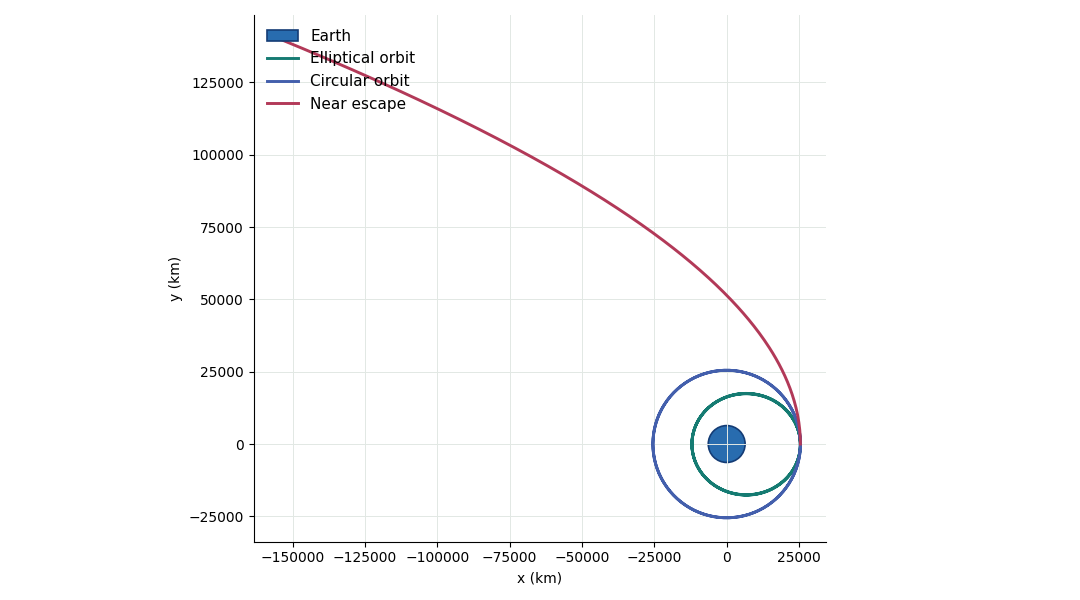
\includegraphics[width=0.95\linewidth]{reference-orbits.png}
\end{center}

The figure shows three saved Julia calculations beginning at four Earth radii.
The launch at $0.80v_c$ is an ellipse, $1.00v_c$ is circular, and the
$1.42v_c$ case is just above escape speed.  The calculations use
velocity-Verlet time stepping, which is a symplectic method and keeps the
long-term behavior of conservative motion well behaved.  Each displayed path
contains 361 samples spanning two circular-orbit periods.

\subsection{Interactive explorer and reproducibility}

The \PMlinkexternal{orbital-gravitation explorer}
{https://images.physicslibrary.org/examples/orbital-gravitation/index.html}
contains 37 reviewed launch speeds from $0.70v_c$ to $1.42v_c$.  Its controls
select and play back saved samples; they do not run Julia, invoke a server-side
calculation, or send user input anywhere.  A test-mass control makes the
mass cancellation visible by changing the force and total energy readings
without changing the selected path.

The downloadable project includes inputs, source, tests, CSV reference data,
the full launch-speed sweep, an environment manifest, and provenance.  To
reproduce the saved output, run:
\begin{verbatim}
julia --startup-file=no --project=. test/runtests.jl
julia --startup-file=no --project=. motion.jl
python3 build.py
python3 verify.py
\end{verbatim}
The model assumes a point-mass Earth and spacecraft.  It omits atmosphere,
Moon and planetary perturbations, Earth oblateness, relativity, thrust,
collisions, and changing spacecraft mass.
